\documentclass{article}

\usepackage{geometry}
\usepackage{amsmath}
\usepackage{graphicx}
\usepackage{listings}
\usepackage{hyperref}
\usepackage{multicol}
\usepackage{fancyhdr}
\pagestyle{fancy}
\hypersetup{ colorlinks=true, linkcolor=black, filecolor=magenta, urlcolor=cyan}
\geometry{ a4paper, total={170mm,257mm}, top=20mm, right=20mm, bottom=20mm, left=20mm}
\setlength{\parindent}{0pt}
\setlength{\parskip}{1em}
\renewcommand{\headrulewidth}{0pt}
\lhead{Competitive Programming - Arkavidia V}
\fancyfoot[CE,CO]{C - \thepage}
\lstset{
    basicstyle=\ttfamily\small,
    columns=fixed,
    extendedchars=true,
    breaklines=true,
    tabsize=2,
    prebreak=\raisebox{0ex}[0ex][0ex]{\ensuremath{\hookleftarrow}},
    frame=none,
    showtabs=false,
    showspaces=false,
    showstringspaces=false,
    prebreak={},
    keywordstyle=\color[rgb]{0.627,0.126,0.941},
    commentstyle=\color[rgb]{0.133,0.545,0.133},
    stringstyle=\color[rgb]{01,0,0},
    captionpos=t,
    escapeinside={(\%}{\%)}
}

\begin{document}

\begin{center}
    \section*{C. Cincin Arvy}

    \begin{tabular}{ | c c | }
        \hline
        Batas Waktu  & 1s \\
        Batas Memori & 512MB \\
        \hline
    \end{tabular}
\end{center}

\subsection*{Deskripsi}

Arvy yang sudah beranjak dewasa pergi ke sebuah toko perhiasan.
Di sana Arvy membeli sebuah cincin untuk hadiah kekasih barunya.
Namun Arvy kurang beruntung pada hari itu.
Sesaat setelah Arvy keluar dari toko, cincin arvy dirampas oleh seorang penjahat.
Kemudian penjahat tersebut berlari melewati rel kereta yang lebarnya $d$ meter.

Arvy ingin melewati rel kereta tersebut, namun di saat yang sama, Arvy melihat sebuah kereta akan melintas.
Kereta tersebut melaju sejauh $v_k$ meter per detik.
Saat ini Arvy sedang berada $y$ meter dari rel dan dapat berlari dengan kecepatan $v_a$ meter per detik.
Kepala kereta berjarak $\sqrt{x^2+y^2}$ meter dari Arvy.
Posisi Arvy, kereta, dan rel dapat digambarkan seperti berikut:

\begin{center}
    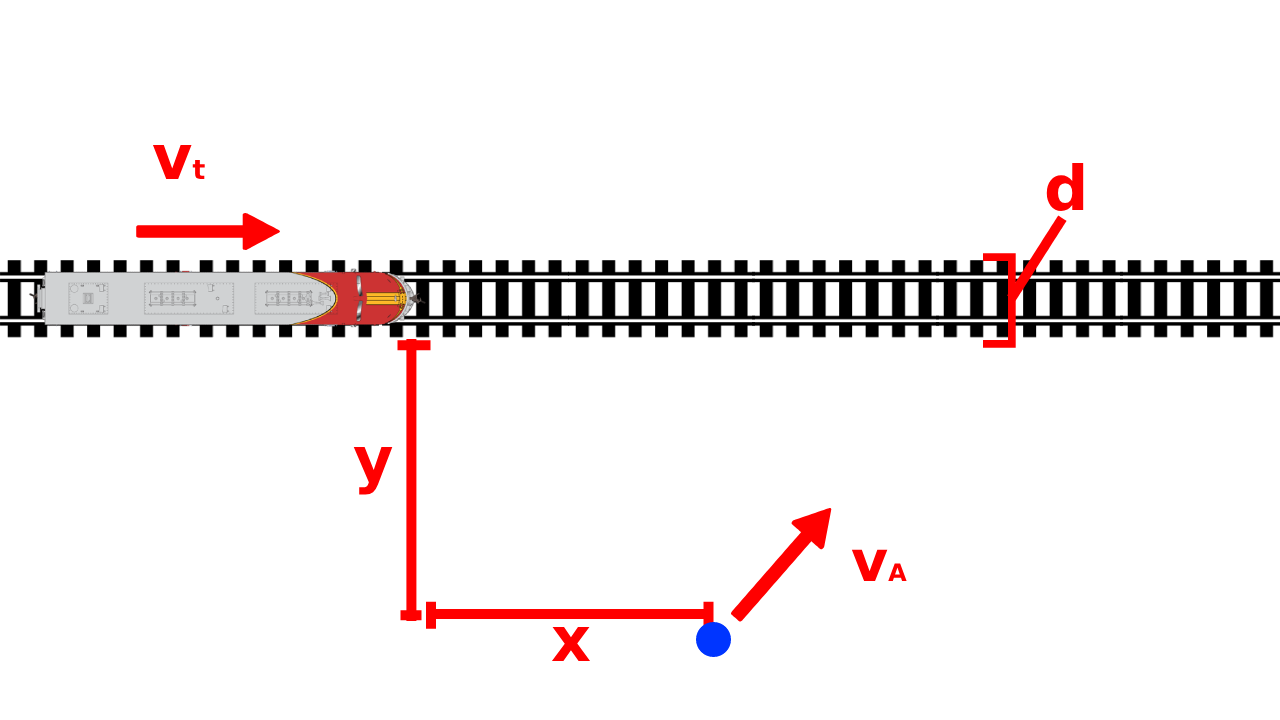
\includegraphics[width=200px]{skema}
\end{center}

Kereta tersebut punya banyak gerbong, jadi kalau Arvy menunggu kereta selesai lewat, pencuri pasti berhasil kabur.
Arvy dapat berlari lurus, bergerak parabola, atau berputar-putar, namun tidak melebihi kelajuan $v_a$ meter per detik.
Apakah Arvy dapat menyebrangi rel sebelum kereta dan mengejar si pencuri cincin?

\subsection*{Format Masukan}
Baris pertama terdiri dari satu bilangan bulat positif $T$ ($1 \leq T \leq 1.000$), menyatakan banyaknya kasus uji.
Setiap kasus uji terdiri dari bilangan $d, x, y, v_k, v_a$ ($1 \leq d, x, y, v_k, v_a \leq 1.000.000.000$) menyatakan lebar rel kereta, jarak horizontal Arvy dengan kereta, jarak vertikal Arvy dengan kereta, kecepatan kereta, dan kecepatan Arvy.

\subsection*{Format Keluaran}
Untuk setiap kasus uji, keluarkan \lstinline{YA} jika Arvy dapat menyebrangi rel, atau \lstinline{TIDAK} jika tidak.

\begin{multicols}{2}
\subsection*{Contoh Masukan}
\begin{lstlisting}
3
1 100 1 5 20
1 10 20 10 5
1 4 6 5 5
\end{lstlisting}
\columnbreak
\subsection*{Contoh Keluaran}
\begin{lstlisting}
YA
TIDAK
YA
\end{lstlisting}
\vfill
\null
\end{multicols}

\newpage
\vspace*{\fill}
\begin{center}
    \textit{Halaman ini sengaja dibiarkan kosong.}
\end{center}
\vspace*{\fill}

\end{document}